\documentclass{article}
\usepackage[utf8]{inputenc}
\usepackage{hyperref}
\usepackage{listings}
\usepackage{multimedia} % to embed movies in the PDF file
\usepackage{graphicx}
\usepackage{comment}
\usepackage[english]{babel}
\usepackage{amsmath}
\usepackage{amsfonts}
\usepackage{wrapfig}
\usepackage{multirow}
\usepackage{verbatim}
\usepackage{float}
\usepackage{cancel}
\usepackage{caption}
\usepackage{subcaption}
\usepackage{mathdots}
\usepackage{/home/cade/Homework/latex-defs}


\title{AMATH 575 Problem Set 2}
\author{Cade Ballew \#2120804}
\date{April 26, 2023}

\begin{document}
	
\maketitle
	
\section{Problem 1}
\subsection{Part a}
We plan to use the following paper:

Brunton, Proctor, and Kutz, Discovering governing equations from data by sparse identification of nonlinear dynamical systems, PNAS, 2016.

Our group consists of myself, Alex Hsu, Catherine Johnston, Kaitlynn Lilly, Ellie Byrnes, and Sara Ichinaga.
\subsection{Part b}
This paper relies on the fact that autonomous dynamical systems express the derivative of the state as a usually simple function of it. Using data of the history of the state and its derivative (or an approximation of it), they fit a sparse function describing the dynamics from a set of candidate functions. 
\subsection{Part c}
The authors find that their method is generally successful at recovering governing equations from data. However, the find that recovery is highly dependent on choosing the correct measurement coordinates and function basis, making the method difficult to apply in general.
\subsection{Part d}
We plan on applying this framework to the water wave problem to see if we can recover asymptotic dynamics (KdV) from data.

\section{Problem 2}
Consider the system

\begin{equation*}
	\left\{\begin{array}{l}
		\dot x= x^2 - y^2  \\
		\dot y = 2 x y 
	\end{array}\right..
\end{equation*}
\subsection{Part a}
By setting the time derivatives equal to zero, we can see that the only fixed point is at $(0,0)$. We then get that the Jacobian at this point is
\[
Df(0,0)=\begin{pmatrix}
	0&0\\0&0
\end{pmatrix}.
\]
Since this is the zero matrix, all vectors are eigenvectors with eigenvalue $0$. Thus, the center manifold is given by $W^C(0,0)=\real^2$ which has dimension 2.
\subsection{Part b}
Consider the manifold $A=\{(x,0):x\in\real\}$ which is clearly 1-dimensional. If $(x,0)\in A$, then the system evolves according to
\begin{equation*}
	\left\{\begin{array}{l}
		\dot x= x^2  \\
		\dot y = 0 
	\end{array}\right.,
\end{equation*}
meaning that it only moves along the $x$-axis, i.e., the invariant manifold $A$.

\section{Problem 3}
Consider the system 
\begin{equation*}
	\left\{\begin{array}{l}
		\dot x= -x \\
		\dot y = y + \alpha x^3 
	\end{array}\right.,
\end{equation*}
for $\alpha>0$. We can again set the time derivatives equal to zero to get that the only fixed point is at $(0,0)$. The Jacobian at this fixed point is given by
\[
Df(0,0)=\begin{pmatrix}
	-1&0\\
	0&1
\end{pmatrix},
\]
which obviously has eigenvalues of $-1,1$ with respective eigenvectors being the unit vectors, meaning that we are already in an eigenbasis and $x$ corresponds to the stable manifold and $y$ the unstable. 

To find the stable manifold, we set $y=h(x)$ and use (4.29) to get
\[
h(x) + \alpha x^3=-h'(x)x.
\]
Solving this via Mathematica, enforcing that $h(0)=0$, we get that the stable manifold is given by 
\[
y=-\frac{\alpha}{4}x^3.
\]

To find the unstable manifold, we set $x=h(y)$ and again use (4.29) to get
\[
-h(y)=h'(y)(y+\alpha h(y)^3).
\]
Solving this via Mathematica, enforcing that $h(0)=0$, we get that $h(y)=0$, so we get that the unsable minfold is given by $W^U(0,0)=\{(0,y):y\in\real\}$.

\section{Problem 4}
Consider linear map on the torus $(x,y) \in \mathbb{T}^2 =  \mathbb{R}^2  /  \mathbb{Z}^2$
\begin{equation*}
	\left\{\begin{array}{l}
		x_{n+1} = x_n + y_n \\
		y_{n+1} = x_n + 2 y_n  
	\end{array}\right..
\end{equation*}
The Jacobian at the fixed point at the origin is given by
\[
Df(0,0)=\begin{pmatrix}
	1&1\\
	1&2
\end{pmatrix}.
\]
Using Mathematica, we find that the stable eigenvalue is given by $\frac{1}{2} \left(3-\sqrt{5}\right)$, so using its eigenvector,
\[
W^S=\text{span}\left\{\left(\frac{1}{2} \left(-\sqrt{5}-1\right),1\right)^T\right\},
\]
and the unstable eigenvalue is given by $\frac{1}{2} \left(\sqrt{5}+3\right)$, so using its eigenvector,
\[
W^U=\text{span}\left\{\left(\frac{1}{2} \left(\sqrt{5}-1\right),1\right)^T\right\}.
\]
Because these vectors are irrational, the manifolds will never self-intersect on the torus, meaning that the will continue to intersect an infinite number of times on the torus.

\section{Problem 5}
Consider the system 
\begin{equation*}
	\left\{\begin{array}{l}
		\dot x= \alpha x^2 -xy \\
		\dot y = -y + x^2 
	\end{array}\right..
\end{equation*}
for all possible real values of $\alpha$. At the fixed point at the origin, the Jacobian is given by
\[
Df(0,0)=\begin{pmatrix}
	0&0\\
	0&-1
\end{pmatrix}.
\]
Clearly, the eigenvalues are $0,-1$ with the standard basis as eigenvectors. Thus, we find the center manifold by setting $y=h(x)$ and using (4.29) to get that
\[
-h(x)+x^2=h'(x)(\alpha x^2 -xh(x)).
\] 
To form a polynomial expansion, we set $h(x)=ax+bx^2$. Plugging this in with Mathematica, we get that the coefficient in $x$ is given by $-a$, so $a=0$. Plugging this in, the $x^2$ coefficient is given by $1-b$, so we get that $b=1$. Thus, up to second order terms, we have that the center manifold is given by $y=x^2$.

To get the approximate flow on this center manifold, we plug in $y=x^2$ to get that 
\[
\dot x= \alpha x^2 -x^3=x^2(\alpha-x),
\]
up to third order in $x$. This looks very similar to Figure 4.6 in Bernard's notes, and we can see from the fact that we have an $x^2$ term which is always nonnegative that when $\alpha\neq0$, the flow is dictated by $\alpha-x$. Thus, the fixed point is unstable when $\alpha\neq0$. When $\alpha=0$, we have $\dot{x}=-x^3$ which implies that the fixed point is stable.

\section{Problem 6}
Consider a map $x_{n+1}=g(x_n)$. A function $I(x)$ should be an integrals for maps if $I(x_{n+1})=I(x_n)$ always holds. Thus the integral is defined by
\[
I(g(x))=I(x).
\]

\section{Problem 7}
Consider the standard map 
\begin{equation*}
	\left\{\begin{array}{l}
		\theta_{n+1}=\theta_{n}+I_{n}-\frac{K}{2 \pi} \sin 2 \pi \theta_{n} \bmod 1 \\
		I_{n+1}=I_{n}-\frac{K}{2 \pi} \sin 2 \pi \theta_{n}
	\end{array}\right.
\end{equation*}
with $K=1$.
\subsection{Part a}
We can verify that this has fixed point (1/2,1) by plugging this to get 
\begin{equation*}
	f_1(1/2,1)=(1/2+1-0)\bmod1=1/2,
\end{equation*}
and 
\begin{equation*}
	f_2(1/2,1)=1-0=1.
\end{equation*}
\subsection{Part b}
To determine the linear stability of this fixed point, we compute the Jacobian
\begin{equation*}
	Df(1/2,1)=\begin{pmatrix}2&1\\1&1\end{pmatrix}.
\end{equation*}
Using Mathematica, we find that this has eigenvalues $\frac{1}{2} \left(\sqrt{5}\pm3\right)$ with eigenvectors. 
\[
\left(\frac{1}{2} \left(1\pm\sqrt{5}\right),1\right)^T.
\]
Thus, the stable eigenspace is given by
\[
\text{span}\left\{\left(\frac{1}{2} \left(1-\sqrt{5}\right),1\right)^T\right\},
\]
and the unstable eigenspace is given by
\[
\text{span}\left\{\left(\frac{1}{2} \left(1+\sqrt{5}\right),1\right)^T\right\}.
\]

\subsection{Part c}
See the attached Jupyter notebook.

\subsection{Part d}
To compute the inverse map, we first get that $I_n=I_{n+1}+\frac{K}{2 \pi} \sin 2 \pi \theta_{n}$. Plugging this into the first equation, we get that $\theta_{n+1}=(\theta_n+I_{n+1})\bmod1$. Thus,
the inverse map is given by
\begin{equation*}
	\left\{\begin{array}{l}
		\theta_{n}=(\theta_{n+1}-I_{n+1}) \bmod 1 \\
		I_n=I_{n+1}+\frac{K}{2 \pi} \sin 2 \pi (\theta_{n+1}-I_{n+1})
	\end{array}\right.
\end{equation*}

\subsection{Part e--g}
See the attached Jupyter notebook.

\section{Problem 8}
Consider the system 
\begin{equation*}
	\left\{\begin{array}{l}
		\dot{x}=-x+a y+x^{2} y \equiv f(x, y) \\
		\dot{y}=b-a y-x^{2} y \equiv g(x, y)
	\end{array}\right.,
\end{equation*}
where $0 < a \le 1/8$, and we only consider nonnegative $x,y$. We first note that the $x$-nullclines are given by $y=x/(a+x^2)$ and the $y$-nullcline is given by $b/(a+x^2)$. Consider a trapping region defined by the inequalities $y\leq b/a$, $x\leq c$, $y\leq-x+b+b/a$ where $c$ is given by the intersection point 
\[
d=-c+b+b/a=\frac{c}{a+c^2},
\]
which does not have a closed form. To show that this is a trapping region, we consider $(x,y)$ along the boundary and show that we flow into the region. First, consider points along the $x$-axis such that $x\leq c$. Then, $\dot y=b>0$ which flows into our region. Now, consider points along the $y$-axis such that $y\leq b/a$. Then, $\dot x=ay\geq0$ which flows into our region. On the line segment where $y=b/a$, $0\leq x\leq b/a$, we have that $\dot y=-bx^2/a^2\leq0$, so we flow into our region. On the line segment $x=c$ with $0\leq y\leq d$, then
\[
\dot{x}\leq-c+(a+c^2)\frac{c}{a+c^2}=0,
\]
so we again flow into our region. Finally, we consider points on the line $y=-x+b+b/a$ such that $d\leq y\leq b/a$, $b\leq x\leq c$. In order to flow into our region, we need that $\dot x+\dot y\leq0$ since this line has slope $-1$. We have that
\[
\dot x+\dot y=-x+a y+x^{2} y+b-a y-x^{2} y=-x+b\leq0.
\]
Thus, we flow into our region on the entire boundary, so this is indeed a trapping region.

Now, we wish apply the Poincar\'e--Bendixson theorem to this region. We can see that the nullclines intersect only at $(b,b/(a+b^2))$, so this is the only fixed point. If we can show that this fixed point strictly repels (all eigenvalues have positive real part), then we can remove it from our region and apply Poincar\'e--Bendixson. We have 
\[
Df(x,y)=\begin{pmatrix}
	-1+2xy&a+x^2\\
	-2xy&-a-x^2
\end{pmatrix}.
\]
Using Mathematica, we plug in the fixed point and find that 
\[
\det(Df(x,y))=a+b^2>0.
\]
Furthermore, Mathematica gives that the trace of this matrix is positive (implying that the eigenvalues have positive real part) when 
\[
\frac{1}{2} (1-2 a)-\frac{1}{2} \sqrt{1-8 a}<b^2<\frac{1}{2} (1-2 a)+\frac{1}{2} \sqrt{1-8 a}.
\]
Thus, when $b$ satisfies this condition, Poincar\'e--Bendixson gives that there must be a stable periodic orbit within this region.

\section{Problem 9}
Consider the system
\begin{equation*}
	\left\{\begin{array}{l}
		\dot{x}=x(a-by) \\
		\dot{y}=y(-c+dx)
	\end{array}\right..
\end{equation*}
where the parameters $a,b,c,d$ are all assumed to be positive, as are $x,y$.
\subsection{Part a}
Setting the time derivatives equal to zero, we can easily see that the fixed points are given by $(0,0)$ and $(c/d,a/b)$. The Jacobian is given by
\[
Df(x,y)=\begin{pmatrix}
	a-by&-bx\\
	dy&-c+dx
\end{pmatrix}.
\]
At $(0,0)$, 
\[
Df(0,0)=\begin{pmatrix}
	a&0\\
	0&-c
\end{pmatrix},
\]
so this fixed point is unstable, because an eigenvalue $a>0$. At $(c/d,a/b)$, 
\[
Df(c/d,a/b)=\begin{pmatrix}
	0&-bc/d\\
	ad/b&0
\end{pmatrix},
\]
so using Mathematica, the eigenvalues are given by $\pm i\sqrt{ac}$. These both have zero real part, so the stability test is inconclusive.

\subsection{Part b}
Setting time derivatives equal to zero, we find that the $x$-nullclines are given by $x=0,y=b/a$ and the $y$-nullclines are given by $y=0,x=c/d$. We plot these along with the phase plots in Mathematica for $a=1,b=2,c=3,d=4$.\\
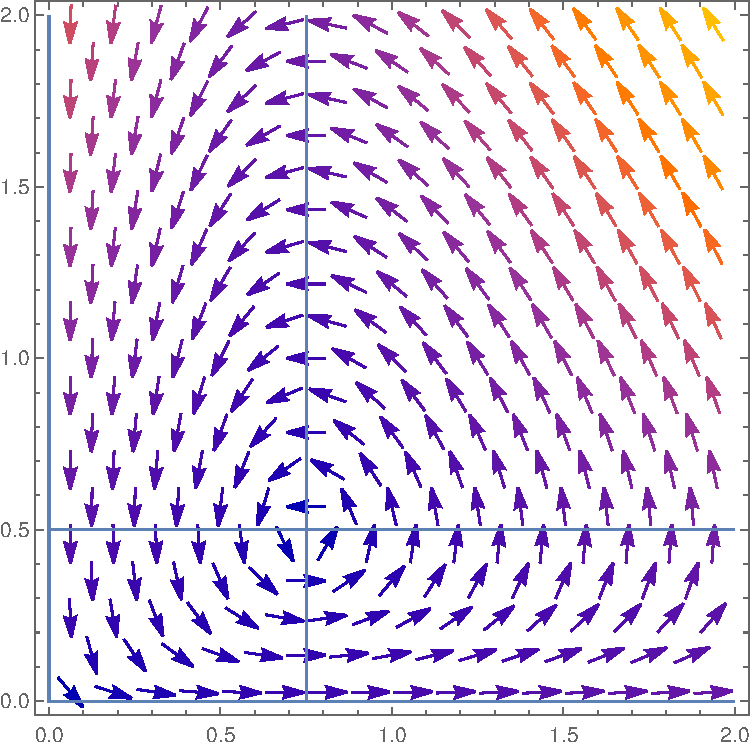
\includegraphics[scale=0.7]{phase_plot.pdf}\\
We infer that the solutions are all cyclic around the fixed point $(c/d,a/b)$.

\subsection{Part c}
Let $L(x,y) = F(x) + G(y)$. Then,
\[
\frac{dL}{dt}=F'(x)\dot{x}+G'(y)\dot{y}=F'(x)x(a-by)+G'(y)y(-c+dx)=0.
\]
Separating,
\[
F'(x)\frac{x}{c-dx}=G'(y)\frac{y}{a-by}=C.
\]
Solving this with Mathematica,
\begin{align*}
F(x)=C (c \log (x)-d x)+c_1,\\
G(y)=C (a \log (y)-b y)+c_2,
\end{align*}
so redefining our constants,
\[
L(x,y)=C_1(c \log (x)-d x+a \log (y)-b y)+C_2.
\]
Using Mathematica, we set $L(c/d,a/b)=0$ to eliminate $C_2$ and get 
\begin{align*}
L(x,y)&=C_1 \left(a \left(-\log \left(\frac{a}{b}\right)\right)+a \log (y)+a-b y-c \log \left(\frac{c}{d}\right)+c \log (x)+c-d x\right)\\&=
C_1\left(a \left(\log \left(\frac{b}{a}y\right)-\frac{b}{a}y+1\right)+c \left(\log \left(\frac{d}{c}x\right)-\frac{d}{c} x+1\right)\right)
\end{align*}
Now, we want to enforce that $L(x,y)>0$ away from the fixed point, which we can do by setting $C_1<0$ since $\log x<x-1$ for all positive $x\neq1$\footnote{This point of equality corresponds to our fixed point in this case.}. For simplicity, we set $C_1=-1$ and get that
\[
L(x,y)=c \left(\frac{d}{c} x-\log \left(\frac{d}{c}x\right)-1\right)+a \left(\frac{b}{a}y-\log \left(\frac{b}{a}y\right)-1\right)
\]

\subsection{Part d}
In part c, we have produced a Lyapunov function around our fixed point $(c/d,a/b)$. Therefore, this fixed point is Lyapunov stable.

\end{document}
